\section{Aircraft ground handling and human factors}
In NLR Air Transport Safety Institute's [insert relation to European Commercial Aviation Safety Team] report, "Aircraft ground handling and human factors" finished in April 2010, on the; "... causal factors which lead to human errors during the ground handling process and create unsafe situations, personal accidents or incidents." (Page 1 of the report); it was found that the largest safety related issues according to operational personnel and management comes from standardization of phraseology on the ramp and human factors such as time pressure, stress, fatigue and communication. This part of the report will describe the detailed findings of the query related to this project and their recommendations to the ground handling companies.

First of all, one of the interesting findings, in the report, was that of what types of accidents happen, and at what relative frequency. In figure \ref{FrequencyOfIncidents}, we can clearly see that incidents that cause operational disruptions, equipment damage and aircraft damage happen at least once a week. As described in section [Freight] damage will not only be costly to repair, it will also most likely cause airplane delays, which can be very expensive for the airlines. Of course operational disrupts also result in delays and therefore loss of income.

\begin{figure}[!h]
\centering
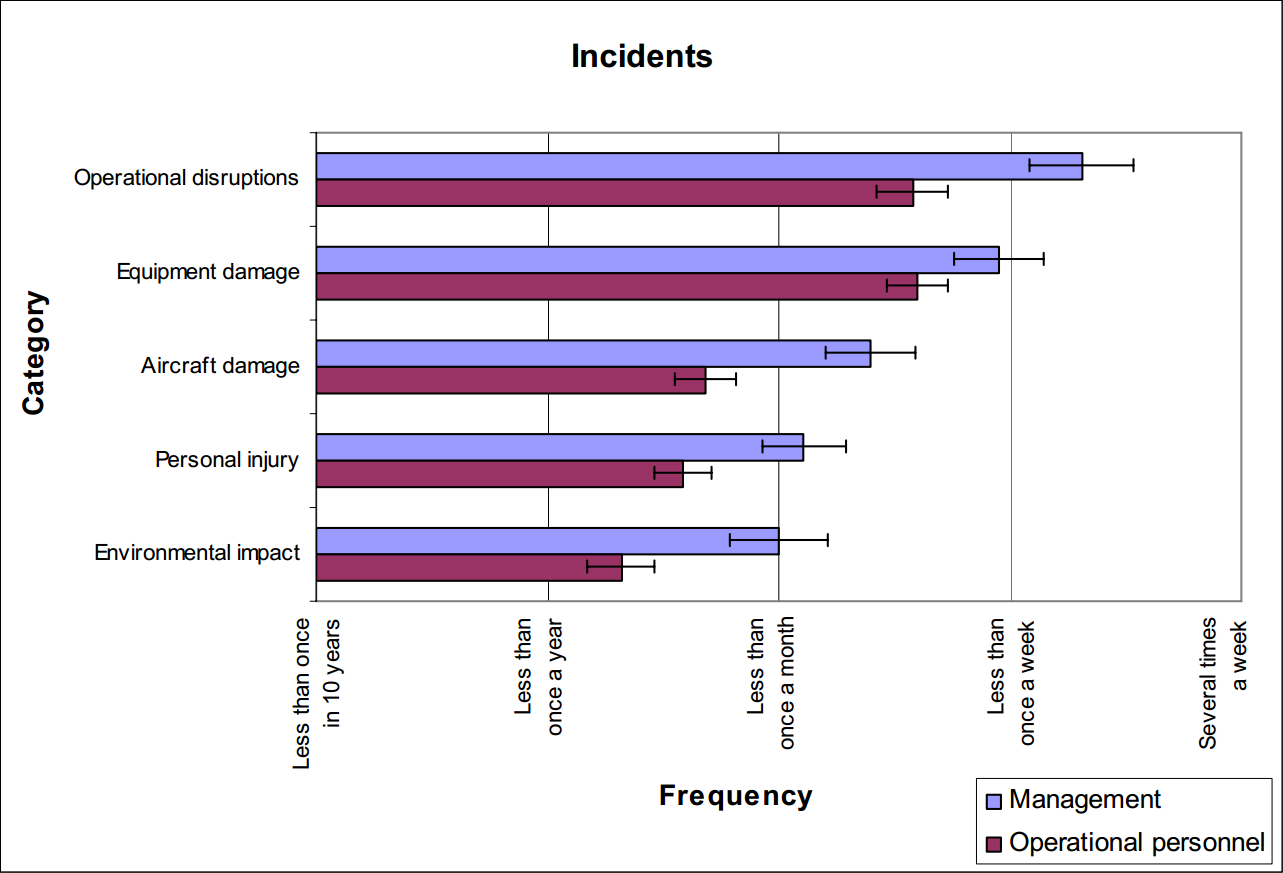
\includegraphics[width=\textwidth]{Grafik/FrequencyOfIncidents}
\caption{The frequency of how often incidents of different categories happens.}
\label{FrequencyOfIncidents}
\end{figure}

To underline this point the study found that delay of incoming and departing flights as a cause of these incidents each happens around once a week (page 29).

[Somebody please write about the "Direct Causes on page 34 of the report, i have no clue!]

Furthermore the survey also researched the contributing factors and how often they contribute to the different kind of accidents. As seen i figure \ref{ContributingFactors} it was found that the two most contributing factors are personal and communication, i.e. mistakes made by people and errors in the communication between people.

\begin{figure}[!h]
\centering
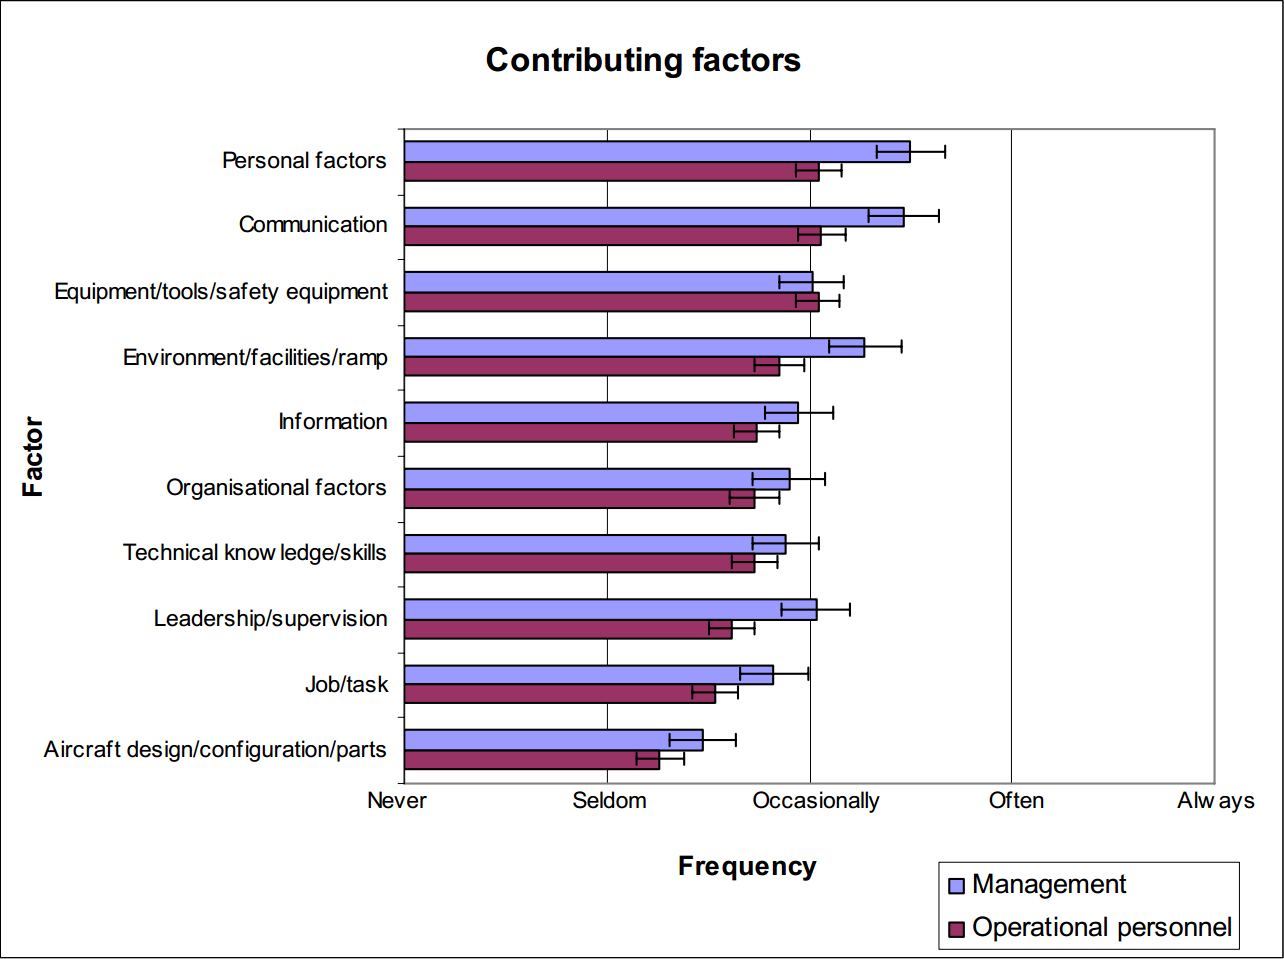
\includegraphics[width=\textwidth]{Grafik/ContributingFactors}
\caption{The contributing factors and how often they contribute to accidents.}
\label{ContributingFactors}
\end{figure}

Next to these two factors Environment/facilities/ramp and Leadership/supervision also recive a high rating from the two groups. 

"With regard to the Environment/facilities/ramp, it may prove to be difficult to mitigate risks resulting from human factors, since aspects related to the environment, facilities and the ramp are mostly managed by the Airport Authorities. With regard to Leadership and supervisionis Management apparently aware that poor leadership or supervision may easily lead to human errors or incident.

Operational personnel provide a higher frequency than Management to the contributing factor of Equipment/tools/safety equipment. This is probably caused by their daily, hands-on experience with the equipment and tools. When compared to the direct causes presented in figure 9, Equipment/tools/safety equipmenthas dropped to the third place, although Operational personnel provide an almost similar frequency to the first three factors in figure 10. For Management, Equipment/tools/safety equipmentdrops to the fifth place. This is due to the fact that there are numerous ways in which equipment or tools may contribute to incidents or human errors."

A very important conclusion, related to our project, in the report is which factors contribute to personal errors and mistakes made by operational personnel and management. As seen in figure \ref{PersonalFactors} it was found that the three major factors contributing to errors and mistakes made by the personnel is time pressure, stress, fatigue and also, very relevant to our project, motivation has a high rating. Especially time pressure is a very high contributor according both operational personnel and management, also because it is expected that both stress and fatigue most likely is a consequence of time pressure. In interviews made with both management and the operational personnel it was found that the reason for fatigue is most likely caused by the ground handling staff having to work double shifts (for different employers) to generate sufficient income. Also these interviews expressed that professional pride to meet the departure time may result in shortcuts have to be taken.

\begin{figure}[!h]
\centering
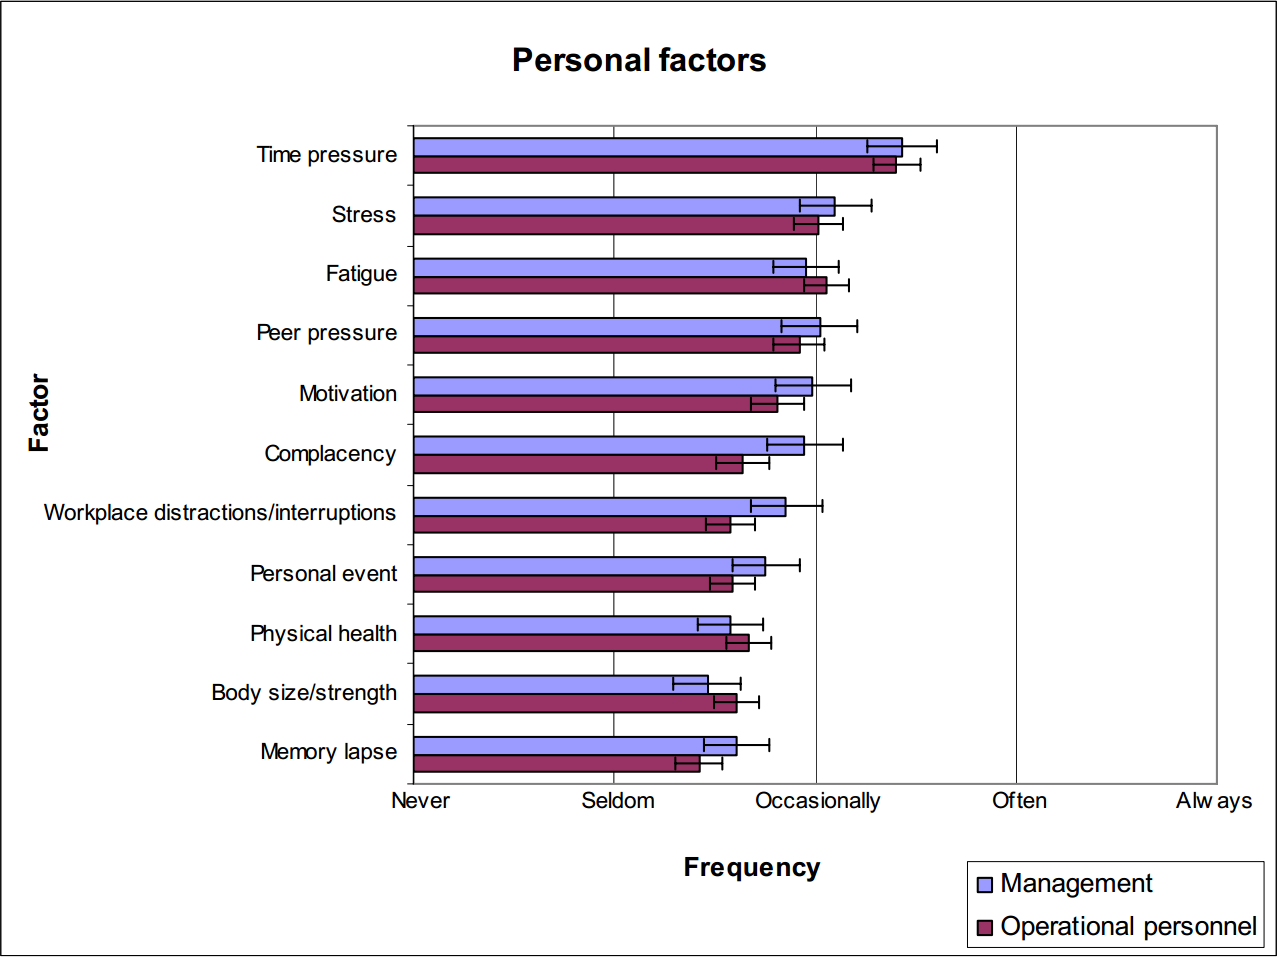
\includegraphics[width=\textwidth]{Grafik/PersonalFactors}
\caption{Breakdown of channels used to book flights.}
\label{PersonalFactors}
\end{figure}

Therefore it is very important to take these contributors into account when considering a solution to prevent and solve the problem which is damage to aircraft, equipment, personal injury, operational disrupts and environmental impact.

"The safety culture of GSP plays an important role in the correct management of time pressure. From the safety culture assessments it was determined that within the safety culture characteristic Awareness, the indicator Attention for safety provided the lowest rating for all participating GSP. This related partially to whether the primary concern is to worksafely or to meet the scheduled departure time. In one of the interviews it was told that Operational personnel often see safety and a fast turnaround to meet the OTD as incompatible, whereas in reality there is always a balance between safety and speed. This balance may differ for each turnaround due to the dynamic environment or different conditions, but when the right balance is found, safety is not compromised."

"Communication between staff and between departments is considered by both Management and Operational personnel as human factors that may contribute to errors. Operational personnel also provide a high frequency for communication between ramp personnel and supervisors, and between supervisors and management. 

Communication of safety issues through the various levels of a GSP is considered important, since is raises the awareness of the role safety plays in the organisation. Communication of safety information makes it possible to learn from safety occurrences and to take proactive action. It is therefore important to promote the development and use of a safety reporting system. This was also one of the findings in the safety culture assessments, in which the safety reporting system was not known or not recognized as such by both Management and Operational personnel."

\begin{figure}[!h]
\centering
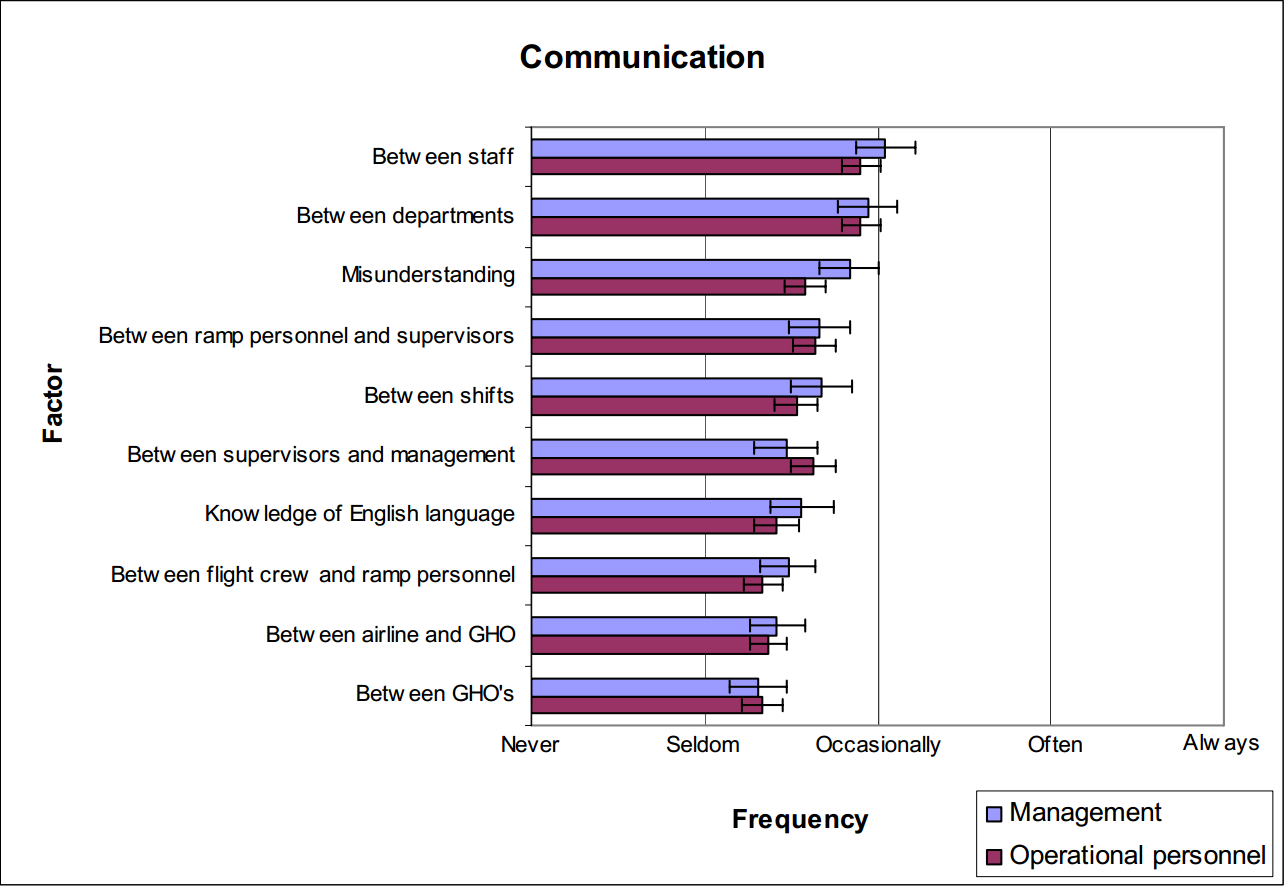
\includegraphics[width=\textwidth]{Grafik/CommunicationalFactors}
\caption{What kind of miscommunication causes incidents and errors.}
\label{CommunicationalFactors}
\end{figure}

According to the survey both management and the operational personnel agree that, when talking about factors surrounding the environment, facilities and ramp, which is the forth highest contributor, rain, wind and snow is the highest contributors. Also humidity, cold and lightning is high contributors. This means that the inefficiency and the rate of accidents, errors and incidents is significantly higher if the weather is bad.

The fifth highest contributor is information, as seen in figure \ref{Information} most information errors contribute nearly similar except  incorrect manufacturer/aircraft documentation, this most like is caused by the fact that ground handling personel is not closly associated with these documents since their company documents already have the procedures and manuals explaining the same.

\begin{figure}[!h]
\centering
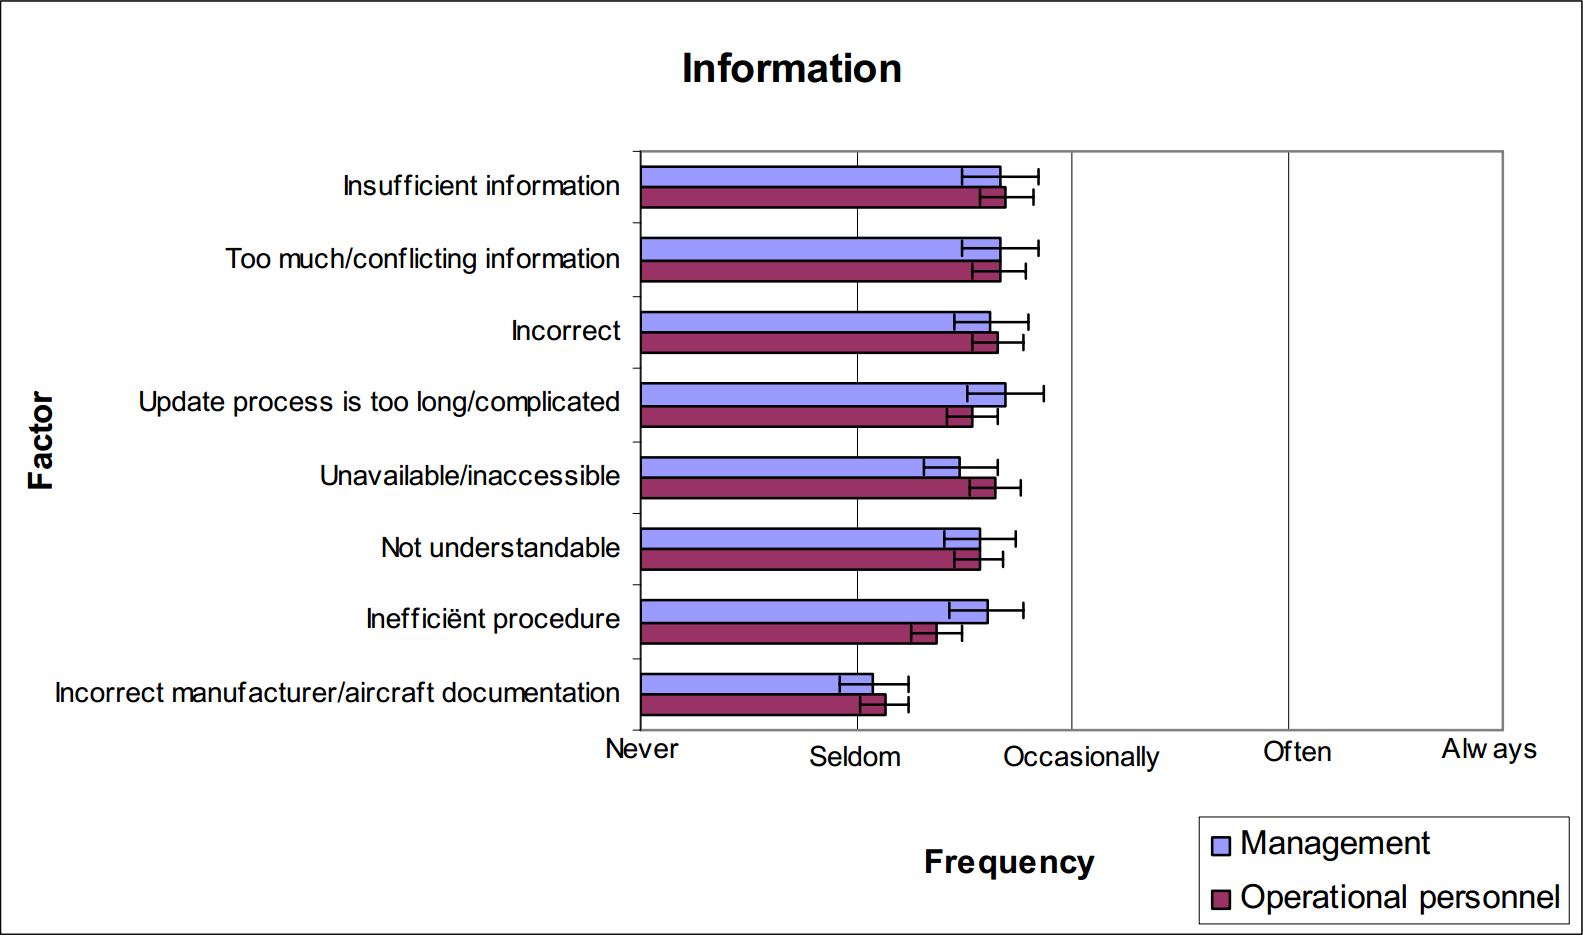
\includegraphics[width=\textwidth]{Grafik/Information}
\caption{Contributors to errors made because of incorrect information.}
\label{Information}
\end{figure}

It is important though to keep in mind that communication can only be effective if the information is correct and these things therefore need to be in order.

"With regard to organisational factors, significant differences between the views of Management and Operational personnel exist in the contributing factors of staffing and adherence to processes and procedures. The opinion that there are insufficient personnel to perform the groundhandling activities is shared by both Management and Operational personnel, but expressed a lot stronger by Operational personnel. In the interviews that concluded the surveys it was expressed that in the current economic tense climate, turnarounds are scheduled with a minimum amount of personnel, with the result that disruptions are increasingly difficult to compensate. This also corresponds with the safety culture assessments, in which the shared impression exists that more experienced personnel are necessary

In the opinion of Management, human errors are occasionally caused by the fact that working processes or procedures are not followed. Operational personnel, on the other hand, provide a much lower frequency to this factor."

\begin{figure}[!h]
\centering
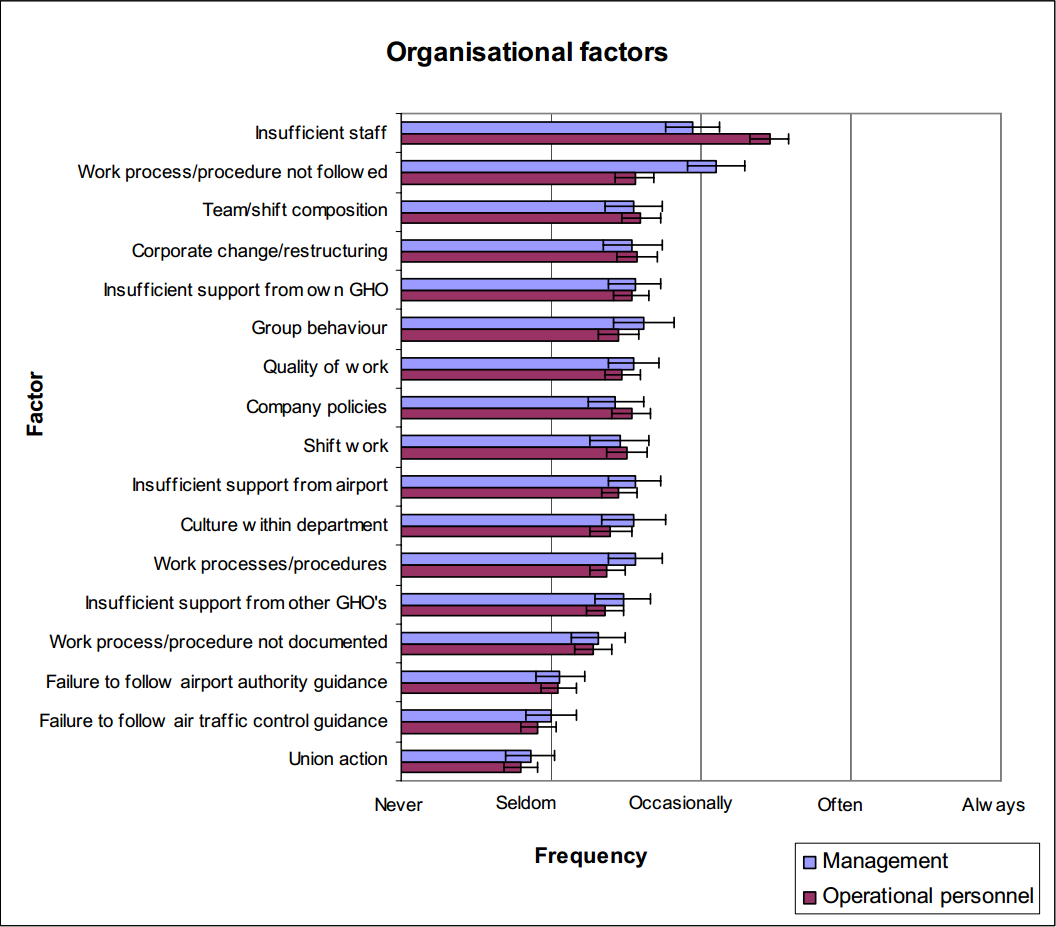
\includegraphics[width=\textwidth]{Grafik/OrganisationalFactors}
\caption{Contributors to bad organization.}
\label{OrganisationalFactors}
\end{figure}

In figure \ref{TechnicalFactors} the important thins is to note that the highest contributor to errors and incidents is task planning. Therefore it is important that the planning of the personel tasks and also skills is done properly to avoid errors and incidents.

\begin{figure}[!h]
\centering
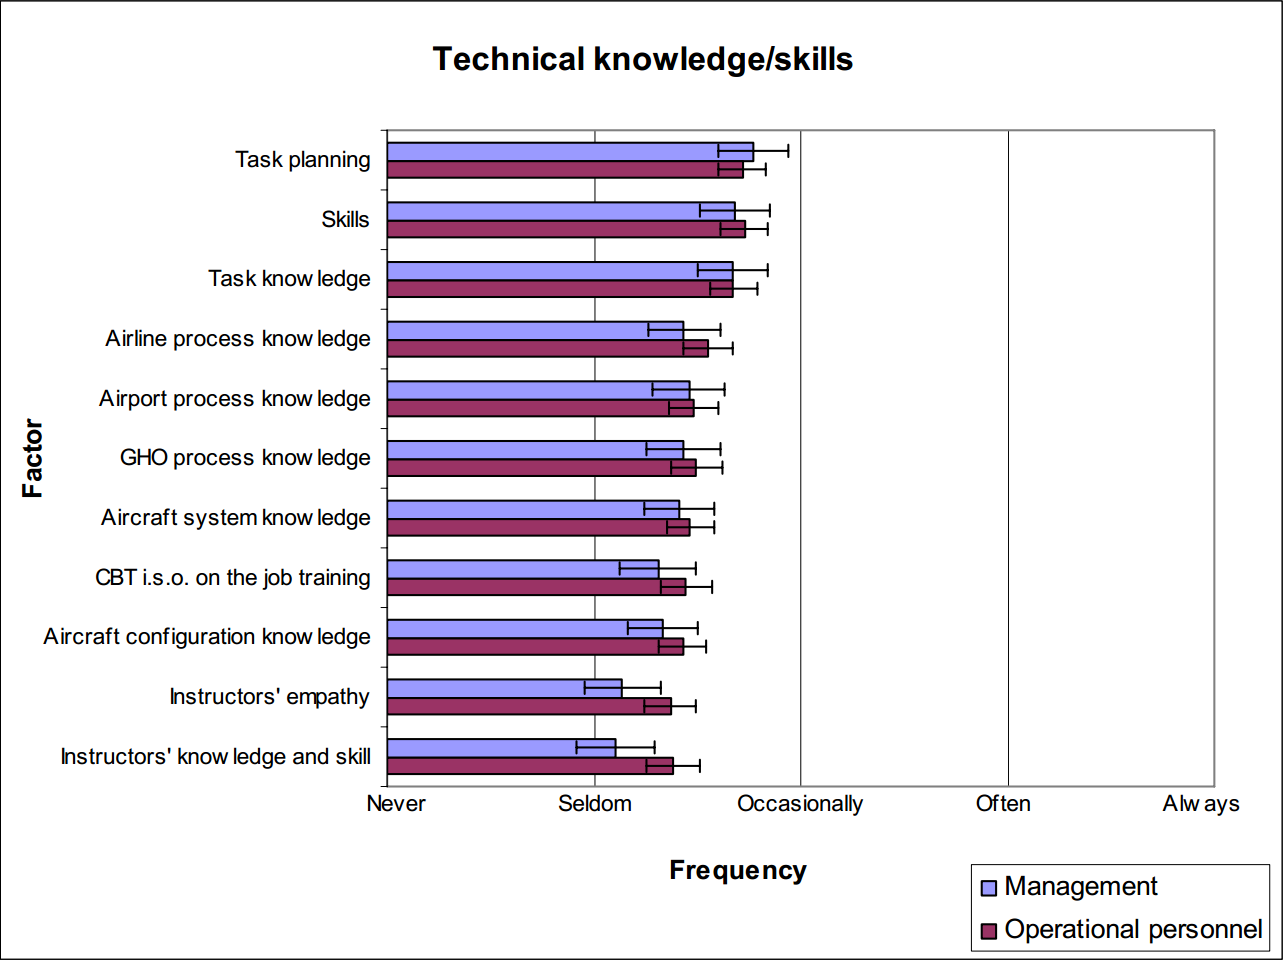
\includegraphics[width=\textwidth]{Grafik/TechnicalFactors}
\caption{Technical contributors to errors and incidents.}
\label{TechnicalFactors}
\end{figure}

The Study also shows that the biggest contributors when talking about leadership, which is the 8th largest contributor to errors, is motivation, prioritization of work and planning. This shows that, when trying to remove the problem discussed in the section, motivating and organizing the workday is very important.